\documentclass[12pt]{article}
\usepackage[margin=1in]{geometry}

% Font and Language (Computer Modern, xelatex)
\usepackage{polyglossia}
\setmainlanguage{greek}
\setotherlanguage{english}
\newfontfamily\greekfont{FreeSerif}
\newfontfamily\greekfonttt{FreeSerif}

% Math
\usepackage{amsmath}

% General
\usepackage{graphicx}
\graphicspath{ {./} }
\usepackage{caption}
\captionsetup{labelsep=none, font={small,it}}
\renewcommand{\thefigure}{}
\usepackage{float}
\usepackage{ragged2e}
\usepackage{fancyhdr}
\usepackage{titlesec}
\usepackage[table]{xcolor}
\usepackage{hyperref}
\usepackage{listings}
\arrayrulecolor{black}

% Listings configuration with colors and frame
\lstset{
    backgroundcolor=\color{white},
    frame=single,
    framesep=4pt,
    framerule=0.5pt,
    rulecolor=\color{gray!50},
    basicstyle=\ttfamily\small,
    keywordstyle=\color{blue}\bfseries,
    stringstyle=\color{red},
    commentstyle=\color{green!50!black},
    numberstyle=\tiny\color{gray},
    numbers=left,
    numbersep=5pt,
    stepnumber=1,
    showstringspaces=false,
    tabsize=4,
    breaklines=true,
    breakatwhitespace=false,
    language=VHDL
}
\hypersetup{
    colorlinks=true,
    linkcolor=blue
}

% Layout
\setlength{\parindent}{0pt}
\setlength{\parskip}{0.5em}

% Title
\title{}
\author{}
\date{}


\begin{document}
    \begin{titlepage}
        \begin{center}

            \begin{minipage}{0.3\textwidth}
                
\includegraphics[width=\linewidth]{../../ntua_logo.png}
            \end{minipage}
            \hfill
            \begin{minipage}{0.65\textwidth}
                \centering
                {\LARGE \textbf{Εθνικό Μετσόβιο Πολυτεχνείο}}\\[0.3cm]
                {\large \textbf{Σχολή Ηλεκτρολόγων Μηχανικών \& Μηχανικών Υπολογιστών}}\\[0.2cm]
                \rule{\linewidth}{0.5pt}\\[0.3cm]
                {\large Εξάμηνο 8\textsuperscript{o}}\\
                {\large \textbf{Ψηφιακά Συστήματα VLSI}}\\
            \end{minipage}

            \vspace{2cm}

            {\Huge \textbf{2η Εργαστηριακή Άσκηση}}\\[1 cm]

            {\Large \textbf{Σχεδίαση Μονάδων Υλικού με την Τεχνική Pipelining}}\\[5 cm]

            {\Large \textbf{Μέλη Ομάδας}}\\[0.5cm]

            \begin{tabular}{rl}
                \textbf{Καβαδάκης Σωτήρης} & 03122035 \\
                \textbf{Κοντοπίδης Δημήτρης} & 03122025 \\
            \end{tabular}

            \vfill

            {\large Αθήνα, Μάρτιος 2026}

        \end{center}
    \end{titlepage}
    \clearpage

% ==============================================================================
% ΕΡΩΤΗΜΑ 1: Σύγχρονος Πλήρης Αθροιστής
% ==============================================================================
\section*{Ερώτημα 1: Σύγχρονος Πλήρης Αθροιστής (Synchronous Full Adder)}
\addcontentsline{toc}{section}{Ερώτημα 1: Σύγχρονος Πλήρης Αθροιστής}

\subsection*{Περιγραφή Κυκλώματος}

Ο Σύγχρονος Πλήρης Αθροιστής (Synchronous Full Adder) είναι ένα ακολουθιακό κύκλωμα που εκτελεί πρόσθεση τριών bits (δύο bits εισόδου και ένα κρατούμενο εισόδου) με τις εξόδους να καταχωρούνται σε flip-flops στη θετική ακμή του ρολογιού. Σε αντίθεση με τον συνδυαστικό Full Adder, οι έξοδοι ενημερώνονται μόνο στη θετική ακμή του σήματος ρολογιού, εισάγοντας καθυστέρηση ενός κύκλου.

Υλοποιήθηκε με περιγραφή συμπεριφοράς (Behavioral) χρησιμοποιώντας process με ευαισθησία στο ρολόι.

Είσοδοι:
\begin{itemize}
    \item \texttt{i\_clk}: Σήμα ρολογιού
    \item \texttt{i\_a}: Πρώτο bit εισόδου
    \item \texttt{i\_b}: Δεύτερο bit εισόδου
    \item \texttt{i\_cin}: Κρατούμενο εισόδου
\end{itemize}

Έξοδοι:
\begin{itemize}
    \item \texttt{o\_sum}: Άθροισμα ($S = A \oplus B \oplus C_{in}$)
    \item \texttt{o\_cout}: Κρατούμενο εξόδου ($C_{out} = (A \cdot B) + (C_{in} \cdot (A \oplus B))$)
\end{itemize}

Ο πίνακας αλήθειας του Synchronous Full Adder:

\begin{table}[H]
    \centering
    \begin{tabular}{|c|c|c|c|c|}
        \hline
        \textbf{i\_a} & \textbf{i\_b} & \textbf{i\_cin} & \textbf{o\_sum} & \textbf{o\_cout} \\
        \hline
        0 & 0 & 0 & 0 & 0 \\
        \hline
        0 & 0 & 1 & 1 & 0 \\
        \hline
        0 & 1 & 0 & 1 & 0 \\
        \hline
        0 & 1 & 1 & 0 & 1 \\
        \hline
        1 & 0 & 0 & 1 & 0 \\
        \hline
        1 & 0 & 1 & 0 & 1 \\
        \hline
        1 & 1 & 0 & 0 & 1 \\
        \hline
        1 & 1 & 1 & 1 & 1 \\
        \hline
    \end{tabular}
    \caption{Πίνακας αλήθειας Synchronous Full Adder}
    \label{tab:sync_fa_truth}
\end{table}

% ------------------------------------------------------------------------------
% 1a) RTL Schematic
% ------------------------------------------------------------------------------
\subsection*{a) Σχεδιάγραμμα Λειτουργίας (RTL Schematic)}

\begin{figure}[H]
    \centering
    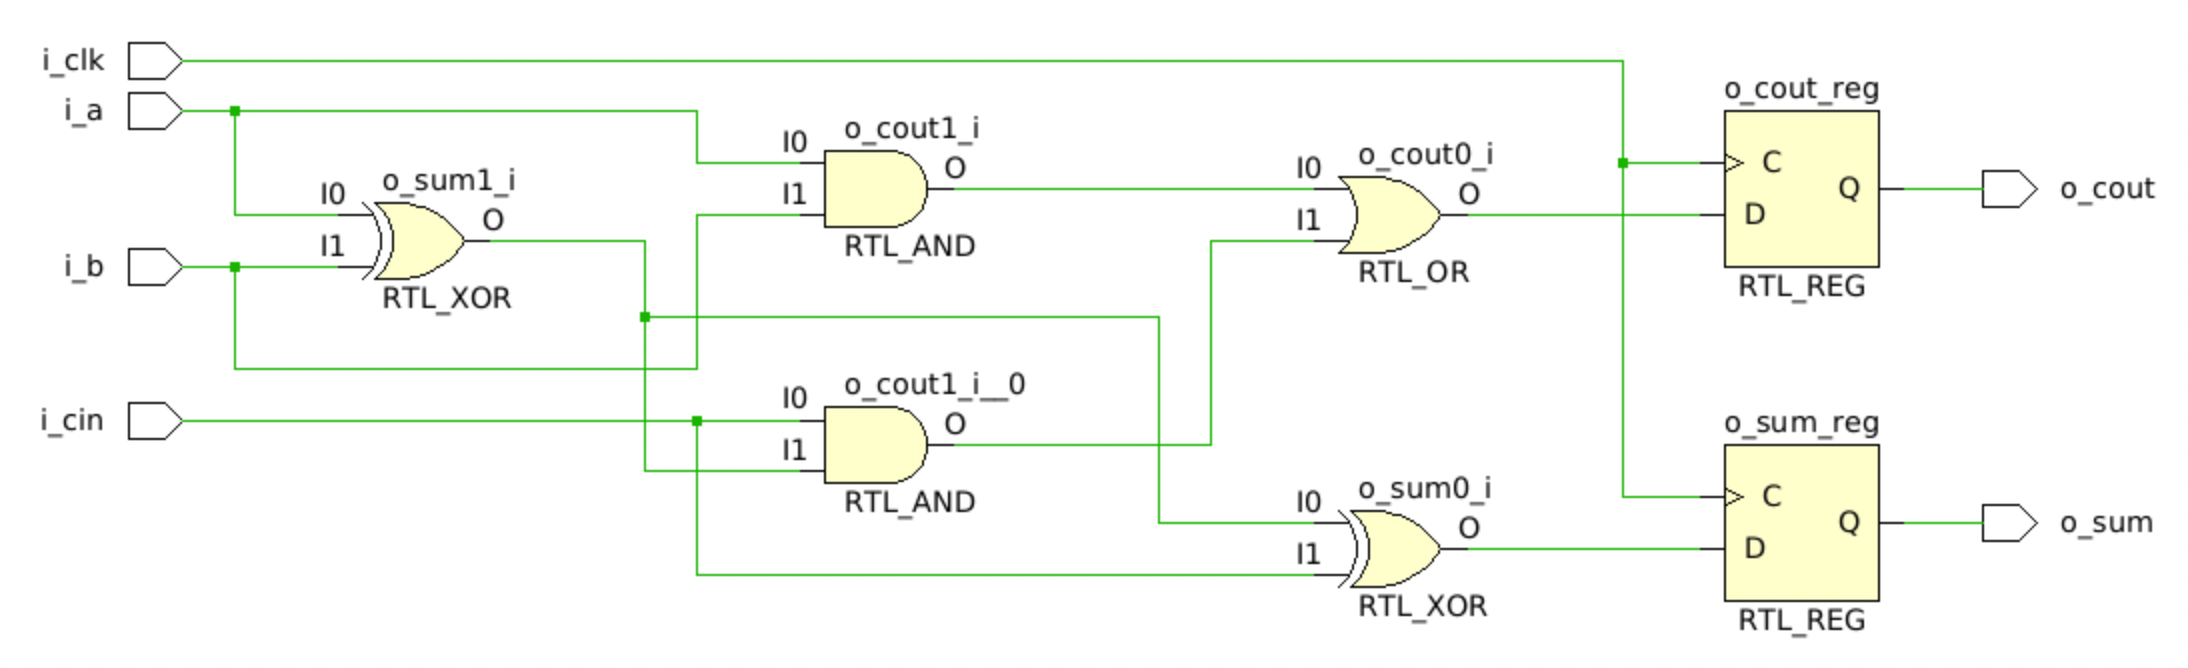
\includegraphics[width=0.9\textwidth]{RTL/sync_full_adder.png}
    \caption{RTL σχηματικό του Synchronous Full Adder}
    \label{fig:sync_fa_rtl}
\end{figure}

Το RTL σχηματικό αποτελείται από:
\begin{itemize}
    \item Μία πύλη \textbf{XOR} για τον υπολογισμό του ενδιάμεσου $A \oplus B$
    \item Δύο πύλες \textbf{AND} για τους όρους $A \cdot B$ και $C_{in} \cdot (A \oplus B)$
    \item Μία πύλη \textbf{OR} για τον υπολογισμό του κρατούμενου $C_{out}$
    \item Μία πύλη \textbf{XOR} για τον υπολογισμό του τελικού αθροίσματος $(A \oplus B) \oplus C_{in}$
    \item Δύο \textbf{RTL\_REG} (flip-flops) που καταχωρούν τα \texttt{o\_sum} και \texttt{o\_cout} στη θετική ακμή του ρολογιού
\end{itemize}

% ------------------------------------------------------------------------------
% 1b) Testbench
% ------------------------------------------------------------------------------
\subsection*{b) Κώδικας VHDL - Behavioral Model}

\begin{lstlisting}[language=VHDL]
library IEEE;
use IEEE.STD_LOGIC_1164.ALL;

entity sync_full_adder is
    Port (
        i_clk : in STD_LOGIC;
        i_a   : in STD_LOGIC;
        i_b   : in STD_LOGIC;
        i_cin : in STD_LOGIC;
        o_sum : out STD_LOGIC;
        o_cout: out STD_LOGIC
    );
end sync_full_adder;

architecture Behavioral of sync_full_adder is
begin
    process(i_clk)
    begin
        if rising_edge(i_clk) then
            o_sum <= (i_a XOR i_b XOR i_cin);
            o_cout <= (i_a AND i_b) OR (i_cin AND (i_a XOR i_b));
        end if;
    end process;
end Behavioral;
\end{lstlisting}

\subsection*{Testbench}

\begin{lstlisting}[language=VHDL]
library IEEE;
use IEEE.STD_LOGIC_1164.ALL;

entity sync_full_adder_tb is
end entity;

architecture tb of sync_full_adder_tb is

    component sync_full_adder is
        Port (
            i_clk      : in  STD_LOGIC;
            i_a        : in  STD_LOGIC;
            i_b        : in  STD_LOGIC;
            i_cin      : in  STD_LOGIC;
            o_sum      : out STD_LOGIC;
            o_cout     : out STD_LOGIC
        );
    end component;

    signal i_Clk        : std_logic := '0';
    signal i_A          : std_logic := '0';
    signal i_B          : std_logic := '0';
    signal i_Carry_in   : std_logic := '0';
    signal o_Sum        : std_logic;
    signal o_Carry_out  : std_logic;

    constant CLK_PERIOD : time := 10 ns;

begin

    DUT: sync_full_adder
        port map (
            i_clk  => i_Clk,
            i_a    => i_A,
            i_b    => i_B,
            i_cin  => i_Carry_in,
            o_sum  => o_Sum,
            o_cout => o_Carry_out
        );

    CLK_PROCESS: process
    begin
        i_Clk <= '0';
        wait for CLK_PERIOD / 2;
        i_Clk <= '1';
        wait for CLK_PERIOD / 2;
    end process;

    STIMULUS: process
    begin
        i_A <= '0'; i_B <= '0'; i_Carry_in <= '0';
        wait for CLK_PERIOD;
        assert (o_Sum = '0' and o_Carry_out = '0')
            report "FAIL: 0+0+0 expected Sum=0, Carry=0";

        i_A <= '0'; i_B <= '0'; i_Carry_in <= '1';
        wait for CLK_PERIOD;
        assert (o_Sum = '1' and o_Carry_out = '0')
            report "FAIL: 0+0+1 expected Sum=1, Carry=0";

        i_A <= '0'; i_B <= '1'; i_Carry_in <= '0';
        wait for CLK_PERIOD;
        assert (o_Sum = '1' and o_Carry_out = '0')
            report "FAIL: 0+1+0 expected Sum=1, Carry=0";

        i_A <= '0'; i_B <= '1'; i_Carry_in <= '1';
        wait for CLK_PERIOD;
        assert (o_Sum = '0' and o_Carry_out = '1')
            report "FAIL: 0+1+1 expected Sum=0, Carry=1";

        i_A <= '1'; i_B <= '0'; i_Carry_in <= '0';
        wait for CLK_PERIOD;
        assert (o_Sum = '1' and o_Carry_out = '0')
            report "FAIL: 1+0+0 expected Sum=1, Carry=0";

        i_A <= '1'; i_B <= '0'; i_Carry_in <= '1';
        wait for CLK_PERIOD;
        assert (o_Sum = '0' and o_Carry_out = '1')
            report "FAIL: 1+0+1 expected Sum=0, Carry=1";

        i_A <= '1'; i_B <= '1'; i_Carry_in <= '0';
        wait for CLK_PERIOD;
        assert (o_Sum = '0' and o_Carry_out = '1')
            report "FAIL: 1+1+0 expected Sum=0, Carry=1";

        i_A <= '1'; i_B <= '1'; i_Carry_in <= '1';
        wait for CLK_PERIOD;
        assert (o_Sum = '1' and o_Carry_out = '1')
            report "FAIL: 1+1+1 expected Sum=1, Carry=1";

        report "All tests passed!";
        wait;
    end process;

end architecture tb;
\end{lstlisting}

\subsection*{Ανάλυση Αποτελεσμάτων Testbench}

Το testbench ελέγχει εξαντλητικά όλους τους $2^3 = 8$ δυνατούς συνδυασμούς εισόδου. Για κάθε συνδυασμό, οι είσοδοι εφαρμόζονται και μετά από έναν κύκλο ρολογιού (10 ns) ελέγχονται οι καταχωρημένες έξοδοι μέσω εντολών assert. Η καθυστέρηση ενός κύκλου αντικατοπτρίζει τη σύγχρονη φύση του κυκλώματος. Εφόσον δεν υπήρξε κάποιο assert error κατά την εκτέλεση, επιβεβαιώθηκε η ορθή λειτουργία.

% ------------------------------------------------------------------------------
% 1c) Critical Path
% ------------------------------------------------------------------------------
\subsection*{c) Κρίσιμο Μονοπάτι (Critical Path)}

\begin{figure}[H]
    \centering
    
\includegraphics[width=0.9\textwidth]{critical_paths/sync_full_adder.png}
    \caption{Κρίσιμο μονοπάτι του Synchronous Full Adder}
    \label{fig:sync_fa_critical}
\end{figure}

Το κρίσιμο μονοπάτι του Synchronous Full Adder είναι από την είσοδο \texttt{i\_a} προς τον καταχωρητή \texttt{o\_sum\_reg/D} με συνολική καθυστέρηση \textbf{1.932 ns} (Logic Delay: 1.132 ns, Net Delay: 0.800 ns). Το μονοπάτι διέρχεται από 2 επίπεδα λογικής (δύο πύλες XOR) και 3 routes. Πρόκειται για μονοπάτι τύπου input-to-register, καθώς οι είσοδοι δεν είναι καταχωρημένες.

% ==============================================================================
% ΕΡΩΤΗΜΑ 2: Pipelined Αθροιστής 4 bits
% ==============================================================================
\newpage
\section*{Ερώτημα 2: Σύγχρονος Αθροιστής 4 bits με Pipeline}
\addcontentsline{toc}{section}{Ερώτημα 2: Σύγχρονος Αθροιστής 4 bits με Pipeline}

\subsection*{Περιγραφή Κυκλώματος}

Ο Pipelined Αθροιστής 4 bits εκτελεί πρόσθεση δύο 4-bit αριθμών με κρατούμενο εισόδου, χρησιμοποιώντας την τεχνική pipeline. Η υλοποίηση βασίζεται σε τέσσερα instances του Synchronous Full Adder (Ερώτημα 1), συνδεδεμένα σε αλυσίδα ripple carry, με επιπλέον pipeline registers για την ευθυγράμμιση των δεδομένων.

Το κύκλωμα μπορεί να δέχεται ένα νέο ζεύγος εισόδων σε κάθε κύκλο ρολογιού και να παράγει ορθό αποτέλεσμα σε κάθε κύκλο μετά από αρχική καθυστέρηση $T_{latency} = 4$ κύκλους.

Είσοδοι:
\begin{itemize}
    \item \texttt{i\_clk}: Σήμα ρολογιού
    \item \texttt{i\_a(3:0)}: Πρώτος 4-bit αριθμός
    \item \texttt{i\_b(3:0)}: Δεύτερος 4-bit αριθμός
    \item \texttt{i\_cin}: Κρατούμενο εισόδου
\end{itemize}

Έξοδοι:
\begin{itemize}
    \item \texttt{o\_sum(3:0)}: 4-bit άθροισμα
    \item \texttt{o\_cout}: Κρατούμενο εξόδου
\end{itemize}

% ------------------------------------------------------------------------------
% 2a) RTL Schematic
% ------------------------------------------------------------------------------
\subsection*{a) Σχεδιάγραμμα Λειτουργίας (RTL Schematic)}

\begin{figure}[H]
    \centering
    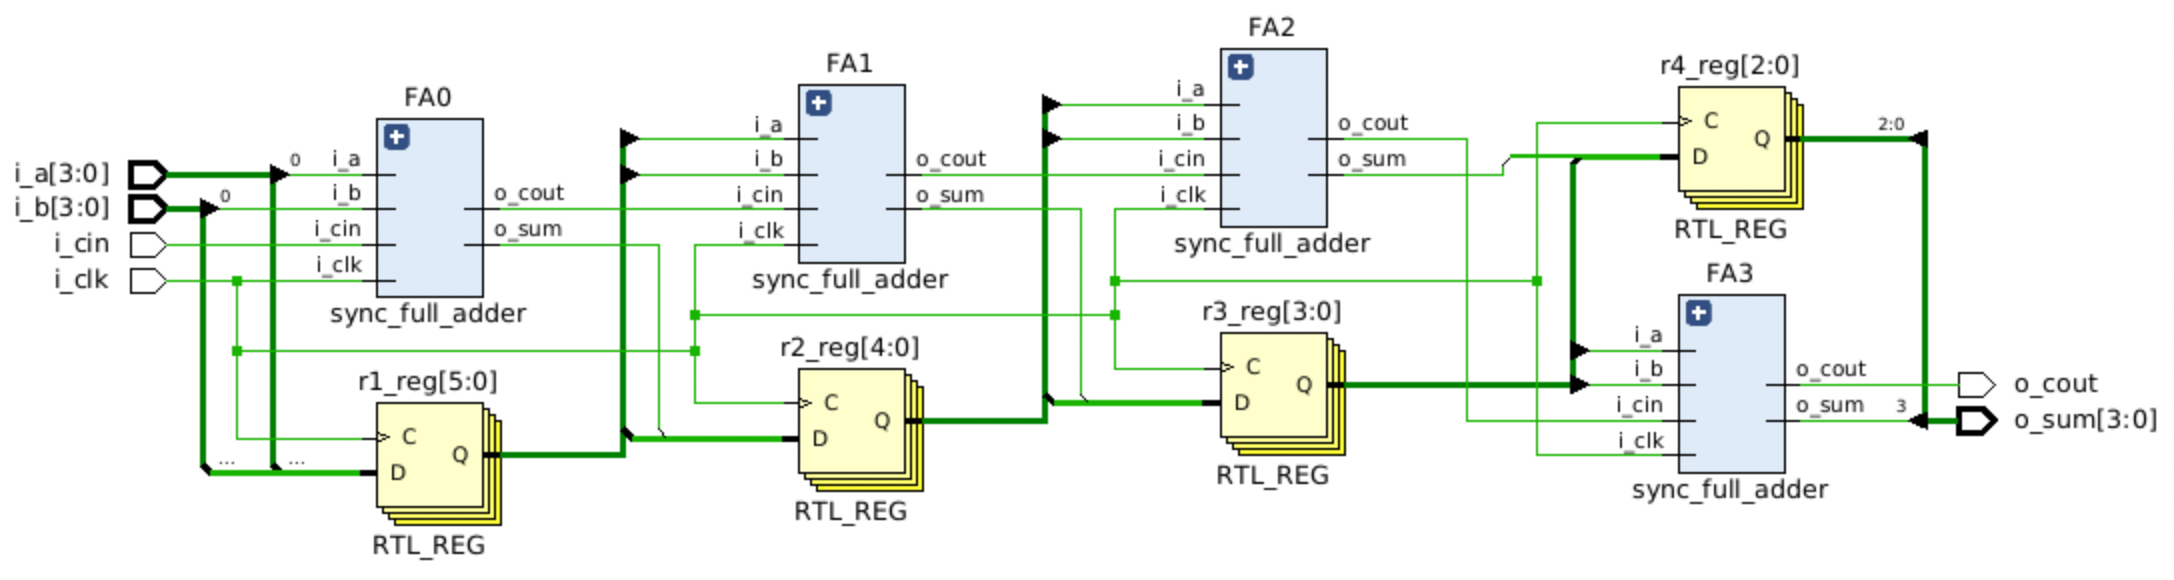
\includegraphics[width=0.9\textwidth]{RTL/pipelined_adder.png}
    \caption{RTL σχηματικό του Pipelined Adder 4 bits}
    \label{fig:pipelined_adder_rtl}
\end{figure}

Η αρχιτεκτονική pipeline χρησιμοποιεί τέσσερα στάδια, ένα για κάθε bit πρόσθεσης. Μεταξύ των σταδίων προστέθηκαν pipeline registers (\texttt{r1}, \texttt{r2}, \texttt{r3}, \texttt{r4}) για τους εξής λόγους:

\begin{itemize}
    \item \textbf{r1 (6 bits)}: Καταχωρεί τα bits εισόδου \texttt{(b3, a3, b2, a2, b1, a1)} που δεν έχουν ακόμη επεξεργαστεί, ώστε να είναι διαθέσιμα στο σωστό στάδιο pipeline.
    \item \textbf{r2 (5 bits)}: Καταχωρεί τα bits \texttt{(b3, a3, b2, a2)} καθώς και το αποτέλεσμα \texttt{s0} από το FA0, ευθυγραμμίζοντάς τα χρονικά με το FA1.
    \item \textbf{r3 (4 bits)}: Καταχωρεί τα bits \texttt{(b3, a3)} και τα αποτελέσματα \texttt{(s1, s0)} για ευθυγράμμιση με το FA2.
    \item \textbf{r4 (3 bits)}: Καταχωρεί τα αποτελέσματα \texttt{(s2, s1, s0)} για ευθυγράμμιση με το FA3.
\end{itemize}

Οι pipeline registers είναι απαραίτητοι γιατί κάθε Full Adder χρειάζεται ένα κύκλο ρολογιού για να υπολογίσει το αποτέλεσμά του. Χωρίς τους ενδιάμεσους καταχωρητές, τα bits εισόδου των ανώτερων βαθμίδων θα είχαν ήδη αλλάξει τιμή πριν χρησιμοποιηθούν, καθώς νέα δεδομένα εισέρχονται σε κάθε κύκλο.

% ------------------------------------------------------------------------------
% 2b) Testbench
% ------------------------------------------------------------------------------
\subsection*{b) Κώδικας VHDL}

\begin{lstlisting}[language=VHDL]
library ieee;
use ieee.std_logic_1164.all;

entity pipelined_adder is
    port (
        i_clk  : in  std_logic;
        i_a    : in  std_logic_vector(3 downto 0);
        i_b    : in  std_logic_vector(3 downto 0);
        i_cin  : in  std_logic;
        o_sum  : out std_logic_vector(3 downto 0);
        o_cout : out std_logic
    );
end pipelined_adder;

architecture Behavioral of pipelined_adder is

    component sync_full_adder is
        port (
            i_clk  : in  std_logic;
            i_a    : in  std_logic;
            i_b    : in  std_logic;
            i_cin  : in  std_logic;
            o_sum  : out std_logic;
            o_cout : out std_logic
        );
    end component;

    -- Carry signals between FA stages
    signal c1, c2, c3 : std_logic;

    -- Sum outputs from each FA
    signal s_int : std_logic_vector(3 downto 0);

    -- Pipeline registers
    signal r1 : std_logic_vector(5 downto 0) := (others => '0');
    signal r2 : std_logic_vector(4 downto 0) := (others => '0');
    signal r3 : std_logic_vector(3 downto 0) := (others => '0');
    signal r4 : std_logic_vector(2 downto 0) := (others => '0');

begin

    -- Pipeline register process
    process(i_clk)
    begin
        if rising_edge(i_clk) then
            r1 <= i_b(3) & i_a(3) & i_b(2) & i_a(2) & i_b(1) & i_a(1);
            r2 <= r1(5) & r1(4) & r1(3) & r1(2) & s_int(0);
            r3 <= r2(4) & r2(3) & s_int(1) & r2(0);
            r4 <= s_int(2) & r3(1) & r3(0);
        end if;
    end process;

    FA0: sync_full_adder
        port map (
            i_clk => i_clk, i_a => i_a(0), i_b => i_b(0),
            i_cin => i_cin, o_sum => s_int(0), o_cout => c1
        );

    FA1: sync_full_adder
        port map (
            i_clk => i_clk, i_a => r1(0), i_b => r1(1),
            i_cin => c1, o_sum => s_int(1), o_cout => c2
        );

    FA2: sync_full_adder
        port map (
            i_clk => i_clk, i_a => r2(1), i_b => r2(2),
            i_cin => c2, o_sum => s_int(2), o_cout => c3
        );

    FA3: sync_full_adder
        port map (
            i_clk => i_clk, i_a => r3(2), i_b => r3(3),
            i_cin => c3, o_sum => s_int(3), o_cout => o_cout
        );

    -- Align all sums
    o_sum(0) <= r4(0);
    o_sum(1) <= r4(1);
    o_sum(2) <= r4(2);
    o_sum(3) <= s_int(3);

end Behavioral;
\end{lstlisting}

\subsection*{Testbench}

\begin{lstlisting}[language=VHDL]
library IEEE;
use IEEE.STD_LOGIC_1164.ALL;
use IEEE.NUMERIC_STD.ALL;

entity pipelined_adder_tb is
end entity;

architecture tb of pipelined_adder_tb is

    component pipelined_adder is
        port (
            i_clk  : in  std_logic;
            i_a    : in  std_logic_vector(3 downto 0);
            i_b    : in  std_logic_vector(3 downto 0);
            i_cin  : in  std_logic;
            o_sum  : out std_logic_vector(3 downto 0);
            o_cout : out std_logic
        );
    end component;

    signal i_clk  : std_logic := '0';
    signal i_a    : std_logic_vector(3 downto 0) := (others => '0');
    signal i_b    : std_logic_vector(3 downto 0) := (others => '0');
    signal i_cin  : std_logic := '0';
    signal o_sum  : std_logic_vector(3 downto 0);
    signal o_cout : std_logic;

    constant CLK_PERIOD : time := 10 ns;

begin

    DUT: pipelined_adder
        port map (
            i_clk => i_clk, i_a => i_a, i_b => i_b,
            i_cin => i_cin, o_sum => o_sum, o_cout => o_cout
        );

    CLK_PROCESS: process
    begin
        i_clk <= '0';
        wait for CLK_PERIOD / 2;
        i_clk <= '1';
        wait for CLK_PERIOD / 2;
    end process;

    STIMULUS: process
        variable expected_cout : std_logic;
    begin
        for a in 0 to 15 loop
            for b in 0 to 15 loop
                for cin in 0 to 1 loop
                    i_a <= std_logic_vector(to_unsigned(a, 4));
                    i_b <= std_logic_vector(to_unsigned(b, 4));
                    if cin = 1 then
                        i_cin <= '1';
                    else
                        i_cin <= '0';
                    end if;
                    wait for 4 * CLK_PERIOD;
                    if (a + b + cin) >= 16 then
                        expected_cout := '1';
                    else
                        expected_cout := '0';
                    end if;
                    assert (o_sum = std_logic_vector(
                            to_unsigned((a + b + cin) mod 16, 4)))
                        and (o_cout = expected_cout)
                        report "FAIL: " & integer'image(a) & "+"
                            & integer'image(b) & "+"
                            & integer'image(cin);
                end loop;
            end loop;
        end loop;
        report "All 512 tests passed!";
        wait;
    end process;

end architecture tb;
\end{lstlisting}

\subsection*{Ανάλυση Αποτελεσμάτων Testbench}

Το testbench ελέγχει εξαντλητικά όλους τους $16 \times 16 \times 2 = 512$ δυνατούς συνδυασμούς εισόδου. Για κάθε συνδυασμό, εφαρμόζονται οι είσοδοι και μετά από 4 κύκλους ρολογιού (η καθυστέρηση pipeline $T_{latency}$), ελέγχεται ότι το αποτέλεσμα είναι ορθό μέσω assert. Εφόσον δεν υπήρξε κάποιο assert error κατά την εκτέλεση, επιβεβαιώθηκε η ορθή λειτουργία του κυκλώματος για όλες τις δυνατές εισόδους.

% ------------------------------------------------------------------------------
% 2c) Critical Path + Comparison
% ------------------------------------------------------------------------------
\subsection*{c) Κρίσιμο Μονοπάτι και Χρονική Ανάλυση (Critical Path \& Timing)}

\begin{figure}[H]
    \centering
    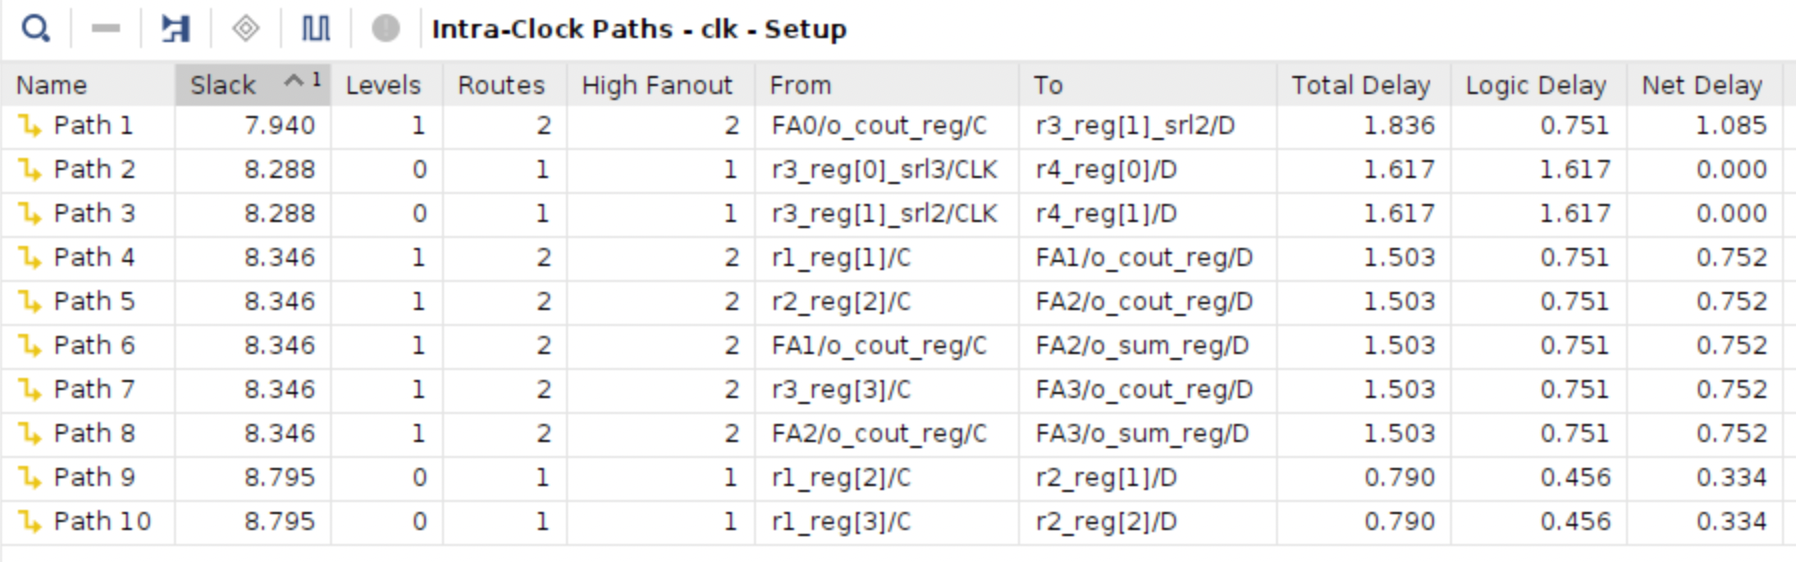
\includegraphics[width=0.9\textwidth]{critical_paths/pipelined_adder_paths.png}
    \caption{Κρίσιμο μονοπάτι του Pipelined Adder}
    \label{fig:pipelined_adder_critical}
\end{figure}

Το κρίσιμο μονοπάτι του Pipelined Adder είναι από τον καταχωρητή \texttt{FA0/o\_cout\_reg/C} προς τον καταχωρητή \texttt{r3\_reg[1]\_srl2/D} με συνολική καθυστέρηση \textbf{2.060 ns} (clock period 10 ns, WNS = 7.940 ns). Το μονοπάτι διέρχεται από 1 επίπεδο λογικής και 2 routes. Πρόκειται για μονοπάτι register-to-register εντός ενός pipeline stage — ακριβώς αυτό που επιτυγχάνει η τεχνική pipeline.

\begin{figure}[H]
    \centering
    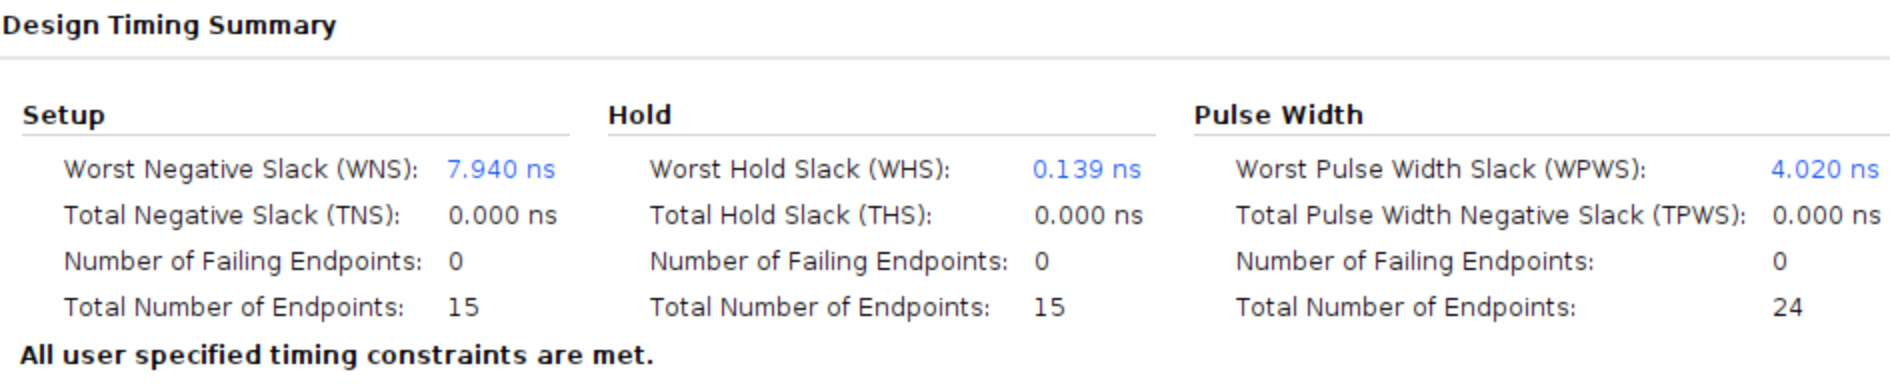
\includegraphics[width=0.9\textwidth]{critical_paths/pipelined_adder_timing.png}
    \caption{Design Timing Summary του Pipelined Adder}
    \label{fig:pipelined_adder_timing}
\end{figure}

Στο Design Timing Summary (Σχήμα \ref{fig:pipelined_adder_timing}) παρατηρούμε ότι όλα τα timing constraints ικανοποιούνται:
\begin{itemize}
    \item \textbf{Setup}: WNS = 7.940 ns, δηλαδή $T_{clk} - T_{critical} = 10.0 - 2.060 = 7.940$ ns slack. Αυτό σημαίνει ότι το κύκλωμα θα μπορούσε να λειτουργήσει σε συχνότητα έως $f_{max} = 1 / 2.060 \text{ ns} \approx 485$ MHz.
    \item \textbf{Hold}: WHS = 0.139 ns $> 0$, άρα δεν υπάρχουν hold violations.
    \item \textbf{Pulse Width}: WPWS = 4.020 ns $> 0$, εντός προδιαγραφών.
    \item Σύνολο 15 setup endpoints και 24 pulse width endpoints, 0 failing — πλήρης επιτυχία.
\end{itemize}

\subsection*{Κατανάλωση Πόρων (Resource Utilization)}

\begin{figure}[H]
    \centering
    
\includegraphics[width=0.8\textwidth]{resource_utilisation/pipelined_adder.png}
    \caption{Resource Utilization του Pipelined Adder}
    \label{fig:pipelined_adder_utilization}
\end{figure}

Από τον πίνακα utilization (Σχήμα \ref{fig:pipelined_adder_utilization}) προκύπτει ότι ο Pipelined Adder χρησιμοποιεί συνολικά \textbf{10 Slice LUTs}, \textbf{21 Slice Registers} (flip-flops), \textbf{15 Bonded IOBs} και \textbf{1 BUFGCTRL}. Η κατανομή ανά instance είναι:
\begin{itemize}
    \item Κάθε \texttt{sync\_full\_adder} (FA0--FA3) χρησιμοποιεί 2 LUTs (ένα για το sum, ένα για το carry) και 1-2 flip-flops (για τις εξόδους \texttt{o\_sum} και \texttt{o\_cout}).
    \item Οι FA2 και FA3 έχουν 2 registers αντί για 1, καθώς τα carry bits τους περνούν μέσω pipeline registers στα επόμενα stages.
    \item Τα υπόλοιπα flip-flops (21 $-$ 6 = 15) αντιστοιχούν στους pipeline registers \texttt{r1}--\texttt{r4} που ευθυγραμμίζουν τα ενδιάμεσα αποτελέσματα μεταξύ stages.
\end{itemize}

\section*{Ερώτημα 3: Πολλαπλασιαστής 4-bit Pipeline με Διάδοση Κρατουμένου}

\subsection*{Περιγραφή Κυκλώματος}

Ο Pipeline RCM (Ripple Carry Multiplier) 4-bit υλοποιεί τον πολλαπλασιασμό δύο 4-bit αριθμών με χρήση τεχνικής pipeline για την επίτευξη υψηλού throughput. Η αρχιτεκτονική βασίζεται στον μετασχηματισμό του παράλληλου πολλαπλασιασμού σε διαδοχικά στάδια πρόσθεσης.

Η δομή του κυκλώματος αποτελείται από:
\begin{itemize}
    \item \textbf{3 Σύγχρονους Παράλληλους Αθροιστές}: Κάθε αθροιστής προσθέτει ένα μερικό γινόμενο (partial product) στο συσσωρευμένο άθροισμα. Ο πρώτος αθροιστής υπολογίζει το άθροιστα $A \times B_0 + A \times B_1$, ο δεύτερος προσθέτει το $A \times B_2$ στο αποτέλεσμα του πρώτου, και ο τρίτoς προσθέτει τo $A \times B_3$. Για τους παράλληλους αθροιστές χρειάζεται να ορίσουμε τα components τους καθώς και το component του full adder.
    \item \textbf{Καταχωρητές Pipeline}: Μεταξύ κάθε σταδίου προστίθενται καταχωρητές (registers) για την απoθήκeυση:
        \begin{itemize}
            \item Των ενδιάμεσων αποτελεσμάτων προσθέσεων
            \item Των τιμών εισόδου A και B
            \item Των LSB bits που μεταφέρονται στο επόμενο στάδιο
        \end{itemize}
    \item \textbf{Τελικός Πολλαπλασιασμός}: Το τελικό bit $B_3$ πολλαπλασιάζεται απευθείας με την είσοδο A και προστίθεται στο τελικό αποτέλεσμα χωρίς επιπλέον pipeline stage.
\end{itemize}

Η αρχιτεκτονική αυτή επιτυγχάνει \textbf{3-κύκλο latency}, καθώς το αποτέλεσμα εξέρχεται μετά από 3 περιόδους ρολογιού από την είσοδο των δεδομένων.

\subsection*{Full Adder Component}
\begin{lstlisting}[language=VHDL]
-------------------------------------------------
-- Synchronous Full Adder (Sequential)
-------------------------------------------------

library IEEE;
use IEEE.std_logic_1164.all;
entity FullAdder is
    port (
        i_A     : in    std_logic;
        i_B     : in    std_logic;
        i_Cin   : in    std_logic;
        o_Sum   : out   std_logic;
        o_Cout  : out   std_logic
    );
end FullAdder;

architecture rtl of FullAdder is
begin
    o_Sum <= i_A XOR i_B XOR i_Cin;
    o_Cout <= (i_A AND i_B) OR (i_Cin AND (i_A XOR i_B));
end rtl;
\end{lstlisting}

\subsection*{Parallel 4-bit Adder Component}

\begin{lstlisting}[language=VHDL]
-----------------------------------------------
-- Synchronous Parallel Adder 
-----------------------------------------------
library IEEE;
use IEEE.STD_LOGIC_1164.ALL;


entity SynchronousParallelAdder is
    Port (
        i_clk  : in  STD_LOGIC;
        i_A    : in  STD_LOGIC_VECTOR (3 downto 0);
        i_B    : in  STD_LOGIC_VECTOR (3 downto 0);
        i_Cin  : in  STD_LOGIC;
        o_S    : out STD_LOGIC_VECTOR (3 downto 0);
        o_Cout : out STD_LOGIC
    );
end SynchronousParallelAdder;

architecture Behavioral of SynchronousParallelAdder is
    component FullAdder is
        Port ( i_a    : in  STD_LOGIC;
               i_b    : in  STD_LOGIC;
               i_cin  : in  STD_LOGIC;
               o_sum  : out STD_LOGIC;
               o_cout : out STD_LOGIC);
    end component;

    signal carry     : STD_LOGIC_VECTOR(3 downto 0);
    
    signal wire_sum  : STD_LOGIC_VECTOR(3 downto 0);
    signal wire_cout : STD_LOGIC;

begin
    FA0: FullAdder port map (i_a => i_A(0), i_b => i_B(0), i_cin => i_Cin, o_sum => wire_sum(0), o_cout => carry(0));
    FA1: FullAdder port map (i_a => i_A(1), i_b => i_B(1), i_cin => carry(0), o_sum => wire_sum(1), o_cout => carry(1));
    FA2: FullAdder port map (i_a => i_A(2), i_b => i_B(2), i_cin => carry(1), o_sum => wire_sum(2), o_cout => carry(2));
    FA3: FullAdder port map (i_a => i_A(3), i_b => i_B(3), i_cin => carry(2), o_sum => wire_sum(3), o_cout => carry(3));
    
    wire_cout <= carry(3);
    
    process(i_clk)
    begin
        if rising_edge(i_clk) then
            -- On clock tick, capture the results in the output registers
            o_S    <= wire_sum;
            o_Cout <= wire_cout;
        end if;
    end process;
    
end Behavioral;
\end{lstlisting}

\subsection*{Synchronous Pipelined 4-bit Ripple Carry Multiplier}
\begin{lstlisting}[language=VHDL]
-------------------------------------------------------
-- Synchronous Pipelined 4-bit Ripple Carry Multiplier
-------------------------------------------------------

library IEEE;
use IEEE.STD_LOGIC_1164.ALL;


entity Pipelined_RCM_4bit is
    Port (
        i_clk  : in  STD_LOGIC;
        i_A    : in  STD_LOGIC_VECTOR (3 downto 0);
        i_B    : in  STD_LOGIC_VECTOR (3 downto 0);
        o_M    : out STD_LOGIC_VECTOR (7 downto 0)
    );
end Pipelined_RCM_4bit;
architecture Structural of Pipelined_RCM_4bit is

    component SynchronousParallelAdder is
        Port (
            i_clk  : in  STD_LOGIC;
            i_A    : in  STD_LOGIC_VECTOR (3 downto 0);
            i_B    : in  STD_LOGIC_VECTOR (3 downto 0);
            i_Cin  : in  STD_LOGIC;
            o_S    : out STD_LOGIC_VECTOR (3 downto 0);
            o_Cout : out STD_LOGIC
        );

    end component;
    -- Intermediate signals (wires) 
    signal wire_pp0, wire_pp1, wire_pp2, wire_pp3 : STD_LOGIC_VECTOR(3 downto 0);
    signal adder_in_A1, adder_in_A2, adder_in_A3  : STD_LOGIC_VECTOR(3 downto 0);
    
    -- Pipeline delay registers for A and B (these hold the state of the inputs as the clock ticks)
    signal A_reg1, A_reg2 : STD_LOGIC_VECTOR(3 downto 0);
    signal B_reg1, B_reg2 : STD_LOGIC_VECTOR(3 downto 0);
    
    -- Pipeline delay registers for the LSBs of the result
    signal LSB_reg1 : STD_LOGIC;
    signal LSB_reg2 : STD_LOGIC_VECTOR(1 downto 0);
    signal LSB_reg3 : STD_LOGIC_VECTOR(2 downto 0);

    -- Adder outputs 
    signal sum1, sum2, sum3 : STD_LOGIC_VECTOR(3 downto 0);
    signal c1, c2, c3       : STD_LOGIC;

begin
    -- Note to self: The combinatorial logic is better to be seperated from the sequential logic
    -- because that way it is easier to understand and implement the design 

    -- Combinatorial Part (generate the inputs for the adders)
    wire_pp0 <= i_A    and (3 downto 0 => i_B(0));    
    wire_pp1 <= i_A    and (3 downto 0 => i_B(1)); 
    wire_pp2 <= A_reg1 and (3 downto 0 => B_reg1(2));  
    wire_pp3 <= A_reg2 and (3 downto 0 => B_reg2(3));  

    -- Adder inputs finalized
    adder_in_A1 <= '0' & wire_pp0(3 downto 1);
    adder_in_A2 <= c1  & sum1(3 downto 1);
    adder_in_A3 <= c2  & sum2(3 downto 1);

    -- Synchronous adder logic which create the partial products
    Adder0: SynchronousParallelAdder port map (
        i_clk => i_clk, i_A => adder_in_A1, i_B => wire_pp1, i_Cin => '0', o_S => sum1, o_Cout => c1
    );
    Adder1: SynchronousParallelAdder port map (
        i_clk => i_clk, i_A => adder_in_A2, i_B => wire_pp2, i_Cin => '0',  o_S => sum2, o_Cout => c2
    );
    Adder2: SynchronousParallelAdder port map (
        i_clk => i_clk, i_A => adder_in_A3, i_B => wire_pp3, i_Cin => '0',  o_S => sum3, o_Cout => c3
    );

    -- Synchronous logic for the pipeline delay registers
    process(i_clk)    
    begin
        if rising_edge(i_clk) then
            A_reg1 <= i_A;
            A_reg2 <= A_reg1;

            B_reg1 <= i_B;
            B_reg2 <= B_reg1;

            -- Delay the LSBs so they reach the final output at the exact same time
            LSB_reg1             <= wire_pp0(0);
            LSB_reg2(1 downto 0) <= sum1(0) & LSB_reg1;
            LSB_reg3(2 downto 0) <= sum2(0) & LSB_reg2(1 downto 0);
            
        end if;
    end process;
    o_M <= c3 & sum3 & LSB_reg3;
    
end Structural;
\end{lstlisting}

\begin{figure}[H]
    \centering
    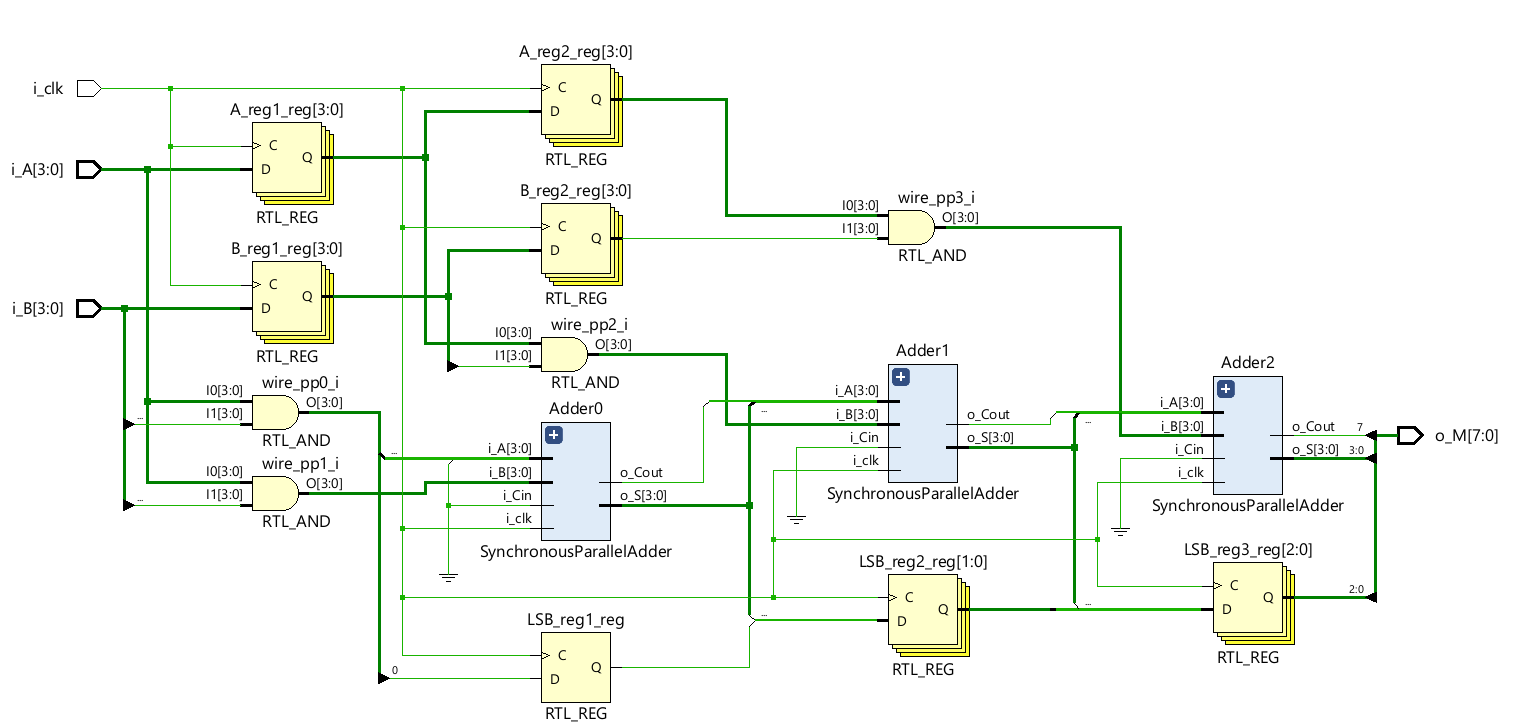
\includegraphics[width=0.9\textwidth]{RTL/pipelined_multiplier.png}
    \caption{RTL δομή του Pipeline RCM 4-bit πολλαπλασιαστή}
    \label{fig:pipelined_multiplier_rtl}
\end{figure}

\subsection*{Περιγραφή Testbench}

Το testbench \texttt{Pipelined\_RCM\_tb.vhd} εκτελεί εξαντλητικό έλεγχο (exhaustive testing) επαληθεύοντας όλους τους 256 συνδυασμούς εισόδων ($2^4 \times 2^4 = 256$). Οι κύριες λειτουργίες του είναι:

\begin{itemize}
    \item \textbf{Παραγωγή Ρολογιού}: Σήμα ρολογιού με περίοδο 10 ns (100 MHz)
    \item \textbf{Διπλός Βρόχος}: Δύο εμφωλευμένοι βρόχοι επαναλαμβάνουν για όλες τις τιμές A (0-15) και B (0-15)
    \item \textbf{Χειρισμός Latency}: Λόγω του pipeline των 3 αθροιστών, τα αποτελέσματα καθυστερούν 3 κύκλους. Χρησιμοποιείται πίνακας \texttt{delay\_array} για την αποθήκευση των αναμενόμενων τιμών με την κατάλληλη καθυστέρηση
    \item \textbf{Assertions}: Για κάθε κύκλο μετά την αρχικοποίηση, ελέγχεται η ορθότητα του αποτελέσματος με assertions
    \item \textbf{Flush}: Μετά την ολοκλήρωση των βρόχων, απαιτούνται 3 επιπλέον κύκλοι για την εκκαθάριση (flush) των δεδομένων που βρίσκονται ακόμα στο pipeline
\end{itemize}

\begin{lstlisting}[language=VHDL]
library IEEE;
use IEEE.STD_LOGIC_1164.ALL;
use IEEE.NUMERIC_STD.ALL;

entity tb_Pipelined_RCM_4bit is
end tb_Pipelined_RCM_4bit;

architecture Behavioral of tb_Pipelined_RCM_4bit is

    -- Component Declaration for the device being tested
    component Pipelined_RCM_4bit is
        Port (
            i_clk  : in  STD_LOGIC;
            i_A    : in  STD_LOGIC_VECTOR (3 downto 0);
            i_B    : in  STD_LOGIC_VECTOR (3 downto 0);
            o_M    : out STD_LOGIC_VECTOR (7 downto 0)
        );
    end component;

    -- Testbench Signals
    signal clk   : STD_LOGIC := '0';
    signal sig_A : STD_LOGIC_VECTOR(3 downto 0) := (others => '0');
    signal sig_B : STD_LOGIC_VECTOR(3 downto 0) := (others => '0');
    signal sig_M : STD_LOGIC_VECTOR(7 downto 0);

    constant clk_period : time := 10 ns;

    -- Verification Variables
    -- Array to store the expected result by 3 cycles
    type delay_array is array (1 to 3) of integer;
    signal expected_pipe : delay_array := (others => 0);
    
    -- Counter to track cycles 
    signal test_cycle : integer := 0; 

begin

    -- Device instance
    DUT: Pipelined_RCM_4bit port map (
        i_clk => clk,
        i_A   => sig_A,
        i_B   => sig_B,
        o_M   => sig_M
    );

    -- Clock generation 
    clk_process : process
    begin
        clk <= '0';
        wait for clk_period / 2;
        clk <= '1';
        wait for clk_period / 2;
    end process;

    -- Exhaustive stimulus with assertions
    stimulus: process
    begin
        
        -- Check all possible combinations for (A,B)
        for i in 0 to 15 loop
            for j in 0 to 15 loop
               
                wait until falling_edge(clk);
                
                -- Check the result after the 3-cycle pipeline latency
                -- Therefore only start checking after 3 cycles have passed
                if test_cycle >= 3 then
                    assert to_integer(unsigned(sig_M)) = expected_pipe(3)
                    report "Mismatched result! " & 
                           "Expected: " & integer'image(expected_pipe(3)) & 
                           ", Got: " & integer'image(to_integer(unsigned(sig_M)))
                    severity error;
                end if;

                -- Delay the expected results by 3 cycles
                expected_pipe(3) <= expected_pipe(2);
                expected_pipe(2) <= expected_pipe(1);
                expected_pipe(1) <= i * j; 
                
                -- Store the new inputs
                sig_A <= std_logic_vector(to_unsigned(i, 4));
                sig_B <= std_logic_vector(to_unsigned(j, 4));
                
                test_cycle <= test_cycle + 1;
                
            end loop;
        end loop;

        -- After the loops finish, the last 3 multiplications are still stuck inside the pipeline.
        -- So we need 3 more clock cycles to get them
        for k in 1 to 3 loop
            wait until falling_edge(clk);
            
            -- Verify the flushing data
            assert to_integer(unsigned(sig_M)) = expected_pipe(3)
            report "Mismatched result during flush! Expected: " & integer'image(expected_pipe(3))
            severity error;
            
            -- Delay the expected results
            expected_pipe(3) <= expected_pipe(2);
            expected_pipe(2) <= expected_pipe(1);
            expected_pipe(1) <= 0; 
            
            sig_A <= (others => '0');
            sig_B <= (others => '0');
        end loop;

        -- Stop the simulation 
        assert false report "Exhaustive Test Completed Successfully! All 256 combinations passed." severity failure;

    end process;

end Behavioral; 
\end{lstlisting}

Η επιτυχής ολοκλήρωση του testbench επιβεβαιώνεται με την απουσία assertion errors.

\subsection*{Κρίσιμο Μονοπάτι και Χρονική Καθυστέρηση}

Το κρίσιμο μονοπάτι στον πολλαπλασιαστή Pipeline RCM διέρχεται μέσω ενός σταδίου πρόσθεσης, δηλαδή μέσω ενός Σύγχρονου Παράλληλου Αθροιστή. Η χρονική καθυστέρηση υπολογίζεται ως:

\[
t_{cp} = t_{co\_FF} + t_{logic\_FA} + t_{routing}
\]

Όπου:
\begin{itemize}
    \item $t_{co\_FF}$: Χρόνος clock-to-output του flip-flop
    \item $t_{logic\_FA}$: Χρονική καθυστέρηση ενός full adder (περιλαμβάνει τη λογική AND για τη δημιουργία partial product και την πρόσθεση)
    \item $t_{routing}$: Χρόνος δρομολόγησης μεταξύ κυκλωμάτων
\end{itemize}

\begin{figure}[H]
    \centering
    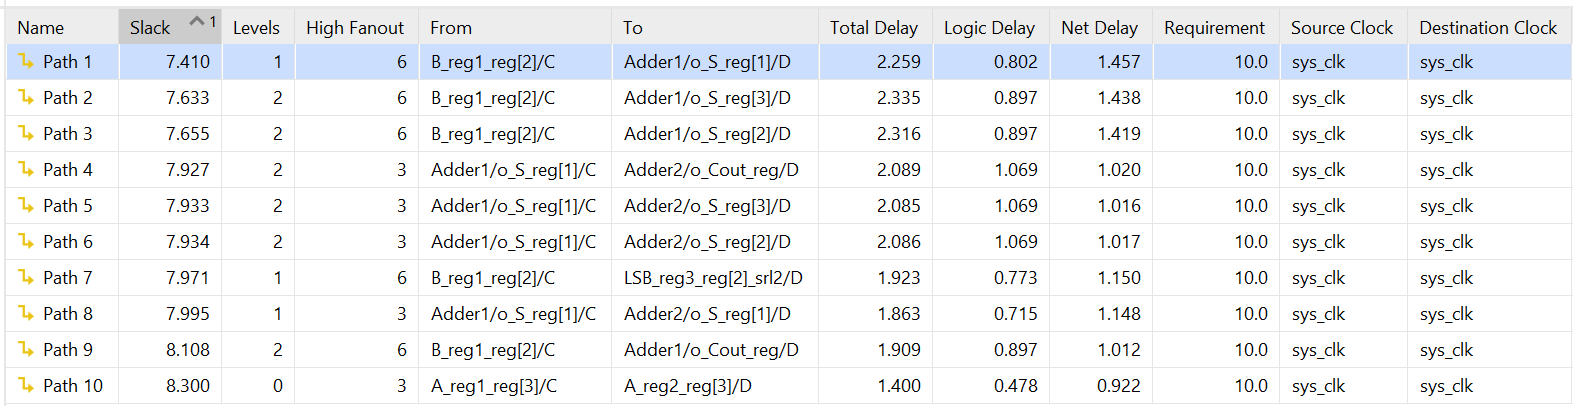
\includegraphics[width=0.9\textwidth]{critical_paths/pipelined_multiplier_paths.png}
    \caption{Κρίσιμα μονοπάτια του Pipeline RCM}
    \label{fig:pipelined_multiplier_paths}
\end{figure}

Από το implementation προκύπτει ότι το κρίσιμο μονοπάτι έχει χρονική καθυστέρηση \textbf{2.259 ns}.

\section*{Ερώτημα 4: Bonus Άσκηση εξοικείωσης με το Zybo}
Σε αυτό το ερώτημα μας δίνεται ο κώδικας blinkled.vhd όπου χρησιμοποιείται ένας μετρητής, του οποίου το MSB ανάβει ένα LED στο Zybo. Ο μετρητής αυξάνεται σε κάθε κύκλο ρολογιού, και το MSB του θα αλλάζει κατάσταση (toggle) κάθε $2^{N-1}$ κύκλους, όπου N είναι το πλήθος των bits του μετρητή. 

Τροποποιούμε αυτό το αρχείο ώστε να πραγματοποιήσουμε μία απεικόνιση και στα 4 leds της πλακέτας που προσομοιώνει την κίνηση ενός βαγονέτου, το οποίο πάει από δεξιά προς τα αριστερά και μετά ξανά προς τα δεξιά. Για να το πετύχουμε αυτό, αξιοποιούμε το MSB του μετρητή ως τρόπος ένδειξης της κατεύθυνσης, το δεύτερο MSB για την εναλλαγή μεταξύ του ζεύγους LEDs που βρίσκεται στο αριστερό μέρος και του ζεύγους που βρίσκεται στο δεξί μέρος και το τρίτο MSB για την επιλογή του LED που θα ανάψει μέσα στο ζεύγος. Με αυτόν τον τρόπο, δημιουργούμε το επιθυμητό εφέ κίνησης.

\subsection*{Κώδικας VHDL για το BlinkLED}
\begin{lstlisting}[language=VHDL]
-------------------------------------------------------------------
-- Blink Single LED Example
-- Digital VLSI Course
-- Microlab <ipapalambrou@microlab.ntua.gr> Ilias Papalamprou
-------------------------------------------------------------------
-- This code implements a simple module that blinks the 4 output  
-- LEDs on Zybo, creating a wagon effect from left to right and back
-- using a single-bit shift register.
--
-- Original code from: 
-- https://digilent.com/reference/learn/programmable-logic/tutorials/zybo-led-demo/start
-------------------------------------------------------------------

library ieee;
use ieee.std_logic_1164.all;
use ieee.numeric_std.all;
use ieee.std_logic_unsigned.all;

entity blink_led is
    generic (
        COUNTER_LIMIT : natural := 27
    );
    port (
        -----------------------------------------------------------
        -- CONTROL SIGNALS
        i_clk   : in    std_logic;
        -----------------------------------------------------------
        -- MAIN SIGNALS
        o_led  : out   std_logic_vector(3 downto 0)
    );
end entity;

architecture behavioral_arch of blink_led is

    signal count_reg : std_logic_vector(COUNTER_LIMIT-1 downto 0) := (others => '0');
    signal a,b,dir : std_logic;
begin
    
    BLINK_LED_PROCESS : process(i_clk)
    begin
        if (rising_edge(i_clk)) then
            count_reg <= count_reg + 1;
        end if;
    end process;
    a <= count_reg(COUNTER_LIMIT-3);
    b <= count_reg(COUNTER_LIMIT-2);
    dir <= count_reg(COUNTER_LIMIT-1);
    o_led(0) <= (a and b)         when dir = '1' else (not a and not b);
    o_led(1) <= (not a and b)     when dir = '1' else (a and not b);
    o_led(2) <= (a and not b)     when dir = '1' else (not a and b);
    o_led(3) <= (not a and not b) when dir = '1' else (a and b);
end behavioral_arch;
\end{lstlisting}

Φυσικά, για να λειτουργήσει ο παραπάνω κώδικας, πρέπει να γίνει κατάλληλη σύνδεση των σημάτων εισόδου και εξόδου στο constraint file του Zybo, ώστε να ορίσουμε τη συχνότητα του ρολογιού και να συνδέσουμε τα LEDs με τα σωστά pins της πλακέτας.

\subsection*{Constraint File (XDC) για το Zybo}
\begin{lstlisting}
# Clock signal
set_property -dict { PACKAGE_PIN L16   IOSTANDARD LVCMOS33 } [get_ports { i_clk }];
create_clock -add -name sys_clk_pin -period 8.00 -waveform {0 4} [get_ports { i_clk }];

# LEDs
set_property -dict { PACKAGE_PIN M14   IOSTANDARD LVCMOS33 } [get_ports { o_led[0] }]; 
set_property -dict { PACKAGE_PIN M15   IOSTANDARD LVCMOS33 } [get_ports { o_led[1] }];
set_property -dict { PACKAGE_PIN G14   IOSTANDARD LVCMOS33 } [get_ports { o_led[2] }];
set_property -dict { PACKAGE_PIN D18   IOSTANDARD LVCMOS33 } [get_ports { o_led[3] }];
\end{lstlisting}


\end{document}
